\documentclass[
%    draft,
]{scrartcl}
%documentclass{scrartcl}
\KOMAoptions{
    fontsize=10pt
}
\setkomafont{pagenumber}{\bfseries\upshape\oldstylenums}
\renewcommand{\titlefont}{\rm\bfseries\LARGE}
\usepackage{
    ifxetex, 
    ifdraft,
    ifthen
}

\ifxetex
  \usepackage{fontspec}
  \usepackage{xunicode}
  \defaultfontfeatures{Mapping=tex-text} % To support LaTeX quoting style
  \setromanfont{Gentium}
\else
  \usepackage[utf8]{inputenc}
  \usepackage[T1]{fontenc}
  \usepackage{lmodern,textcomp}
\fi

\usepackage{
%    standalone,
%    lastpage,
    geometry,
    scrpage2,
%    setspace,
    amsmath,
    caption,
    calc,
%    floatrow,
}
\usepackage{
%    xcolor,
    graphicx,
    tikz,
    chemfig
}
\usepackage[final]{listings}
\usepackage[version=3]{mhchem}
\usepackage[update,verbose=false]{epstopdf}
\usepackage[colorinlistoftodos,obeyDraft]{todonotes}
\usepackage{hyperref}


% Set the geometry
\geometry{
    paper = a4paper,
    top=3cm,
    bottom=4cm,
    footskip=1cm,
    marginparwidth=3.5cm,
    headsep=1cm
}
\ifoptiondraft{
\geometry{inner=1.5cm, outer=4cm}
}{
\geometry{inner=3.0cm, outer=2.5cm}
}

%\onehalfspacing

% Setup hyperref
\hypersetup{
    colorlinks,
    urlcolor=blue,
    breaklinks
}

\usetikzlibrary{
    arrows,
    decorations.pathmorphing,
    backgrounds,
    positioning,
    fit,
    petri
}

% Define collors
\definecolor{myyellow}{HTML}{FFFAC9}
\definecolor{myyellowl}{HTML}{FFFBDD}

% Define lstlisting env
\lstset{
    language=[LaTeX]TeX,
    backgroundcolor=\color{myyellowl},
    numbers=left,
    numberstyle=\footnotesize,
    breaklines=true,
    breakatwhitespace=true,
    print=true
}

% Renew 2 styles
\renewpagestyle{plain}{{}{}{}}{{}{}
{\hfill\pagemark{}}}
\renewpagestyle{headings}{{}{}{}}{{}{}
{\hfill\pagemark{}}}

% Set the headings page style
\pagestyle{headings}

% Text mode commands
\newcommand{\uurl}[2]{\href{#1}{#2}\footnote{The URL is \url{#1}}}
\newcommand{\ftype}[1]{\texttt{.#1}}
\newcommand{\fname}[2]{\texttt{#1.#2}}
\newcommand{\pkg}[1]{\texttt{#1}}
\newcommand{\env}[1]{\texttt{#1}}
\newcommand{\cmd}[1]{\texttt{\textbackslash{}#1}}
\newcommand{\usepkg}[2]{
    \texttt{\textbackslash{}usepackage%
    \ifthenelse{\equal{#2}{}}{}{[#2]}\{#1\}}}
\newcommand{\comment}[1]{}

% New commands which ease the work. Units and relative uncertainties
\newcommand{\unit}[1]{\ensuremath{\, \mathrm{#1}}}
\newcommand{\rel}[1]{\ensuremath{ \cfrac{\Delta #1}{#1}}}
\newcommand{\eten}[1]{\ensuremath{ \times 10^{#1}}}
\newcommand{\DP}[2]{\ensuremath{\cfrac{\partial #1}{\partial #2}}}
\newcommand{\DD}[2]{\ensuremath{\cfrac{\mathrm{d} #1}{\mathrm{d} #2}}}
\newcommand{\dd}[1]{\ensuremath{\mathrm{d}#1}}

% Alter some LaTeX defaults for better treatment of figures:
    % See p.105 of "TeX Unbound" for suggested values.
    % See pp. 199-200 of Lamport's "LaTeX" book for details.
    %   General parameters, for ALL pages:
    \renewcommand{\topfraction}{0.9}    % max fraction of floats at top
    \renewcommand{\bottomfraction}{0.8} % max fraction of floats at bottom
    %   Parameters for TEXT pages (not float pages):
    \setcounter{topnumber}{2}
    \setcounter{bottomnumber}{2}
    \setcounter{totalnumber}{4}     % 2 may work better
    \setcounter{dbltopnumber}{2}    % for 2-column pages
    \renewcommand{\dbltopfraction}{0.9} % fit big float above 2-col. text
    \renewcommand{\textfraction}{0.07}  % allow minimal text w. figs
    %   Parameters for FLOAT pages (not text pages):
    \renewcommand{\floatpagefraction}{0.7}      % require fuller float pages
    % N.B.: floatpagefraction MUST be less than topfraction !!
    \renewcommand{\dblfloatpagefraction}{0.7}   % require fuller float pages

\captionsetup{
    format          = plain,        %
    labelformat     = simple,       %
    labelsep        = period,       %
    justification   = default,      %
    font            = default,      %
    labelfont       = {bf,sf},      %
    textfont        = default,      %
    margin          = 0pt,          %
    indention       = 0pt,          %
    parindent       = 0pt,          %
    hangindent      = 0pt,          %
    singlelinecheck = false         %
}

\renewcommand{\thefigure}{\oldstylenums{\arabic{figure}}}

\setatomsep{5mm}
\setbondoffset{.5mm}
\setcrambond{2.5pt}{1pt}{2pt}
\setbondstyle{thick}
\renewcommand*\printatom[1]{{\footnotesize\ensuremath{\mathsf{#1}}}}


% Custom things
\graphicspath{{./figs/}}
\newlength{\tikzunit}
\newcommand{\scale}{.8}
\newcommand{\compx}[1]{\textbf{#1}}


\title{Getting good quality graphics inside a \LaTeX{} document}
\author{Ignas Anikevičius}

% ----------------------------------------------------------------------
\begin{document}
% ----------------------------------------------------------------------

\maketitle
\tableofcontents
\listoftodos

% ----------------------------------------------------------------------
\clearpage
\section{Introduction}
% ----------------------------------------------------------------------

%
For publications and scientific articles, reports and thesis the most important
    thing is to make well looking graphics. 
%
For that there are several guidelines, which help one to get his figures look
    professionally, but at the same time not to overdo things as there is a
    limit of how good the quality has to be.

\begin{enumerate}
    \item Use vector graphics as much as possible. Especially where there is a
        lot of text in the figure. But remember, if you 'convert' a jpg to eps
        or svg or any other vector graphics format, you will \textbf{not} gain
        any quality. More on this, please use
        \href{http://www.google.co.uk}{Google}
    \item If you have to use raster graphics, please select \ftype{png} format as
        a better alternative where possible
    \item If you use raster graphics, do not exceed the final resolution of the
        picture to more than 600dpi as most of the printers are printing at
        300dpi or 600dpi, so anything more than that might just be wasted time
        while waiting the figure to be rendered. Of course if you have a good
        reason why you need more than 600dpi, then go ahead.
    \item Have a high quality copy of your figure somewhere in your computer.
        This is because while converting from one format to another one can
        \textbf{not} improve the quality.
\end{enumerate}

If you feel that you have not found enough information on the graphics usage in
\LaTeX, please refer to these websites:
\begin{itemize}
    \item
        \href{https://secure.wikimedia.org/wikibooks/en/wiki/LaTeX/Floats,_Figures_and_Captions}{Floats,
        Figures and Captions}
    \item
        \href{https://secure.wikimedia.org/wikibooks/en/wiki/LaTeX/Importing_Graphics}{Importing
        Graphics}
    \item
        \href{https://secure.wikimedia.org/wikibooks/en/wiki/LaTeX/Creating_Graphics}{Creating
        Graphics}
\end{itemize}

% ----------------------------------------------------------------------
\clearpage
\section{Inserting a simple figure}
% ----------------------------------------------------------------------

%
Inserting a figure is a really easy task and it can be accomplished with the
    following code. 
%
Note, that there is an option to the \verb|\includegraphics| command which
    scales the image, so that its width would not exceed the text width.
%
\lstinputlisting{fig1.tex}
%
And our figure will look as follows:
%
\begin{figure}[H]
    \begin{center}
        \includegraphics{plot3.eps}
    \end{center}
    \caption{First plot}
    \label{fig:figure1}
\end{figure}


% ----------------------------------------------------------------------
\clearpage
\section{Directory setting for graphics, their formats and \LaTeX{} compilers}
% ----------------------------------------------------------------------

%
The most convenient way nowadays to produce documents from \LaTeX{} source code
    is to use the \verb|pdftex| or \verb|pdflatex| compiler. 
%
It is because it produces a \ftype{pdf} file directly and you do not need to
    convert the \ftype{ps} file every time before viewing it with a viewer.
%
Also with \verb|pdflatex| you can use more graphics formats:
%
\begin{description}
    \item[\ftype{pdf}] This is the native graphics vector format for this compiler
    \item[\ftype{eps}] This format also can be used with pdflatex, but you need to use
        the \verb|epstopdf| package, which will convert them to
        \ftype{pdf} files on the fly. There are also options to make the
        conversion only when the \ftype{eps} figures are changed, which speeds
        up everything
        substantially.
    \item[\ftype{png}, \ftype{jpg}] At last you can use this format too if you need to import
        raster graphics into your document, which might ease a lot of things.
\end{description}

%
For all these features, one should use the \verb|graphicx| package as this is
    the recommended way to do it. 
%
What is more, this packages provides some other useful commands. 
%
You can tell it where to search for figures by issuing the following command
    (note the / symbol after the directory name):
%
\begin{lstlisting}
\graphicspath{{./path/to/your/directory/}{./second/directory/}}    
\end{lstlisting}
%
The symbols \verb|./| mean, that the top directory is where the \ftype{tex} file
    is located. 
%
So if you have the following directory structure:
%
\begin{lstlisting}
some document
    |-figures
    |-mytexfile.tex
\end{lstlisting}
    %
    you will need to issue \verb|\graphicspath{{./figures}|. 
%
The preamble of this file contains the following lines:
%
\begin{lstlisting}
\usepackage[pdftex]{graphicx}
\graphicspath{{./figs/}}
\usepackage[update,verbose=false]{epstopdf}
\end{lstlisting}
%
There is one thing, which you should be aware of, that is all names should not
    contain white-space as they are known to break on some setups.
%
So if it is working for you, it might not work for others.

%
The options for the \verb|epstopdf| package mean, that it will convert the
    \ftype{eps} graphics only when they are updated and it will not output any
    errors.

% ----------------------------------------------------------------------
\clearpage
\section{Overlaying a figure with \LaTeX{} code}
% ----------------------------------------------------------------------

%
There are many ways how to overlay \LaTeX{} macros on top of a figure and I will
    present some of them in this section.
%
These are using the native \env{picture} environment, whereas the other ways
    rely on either of \pkg{XyPic}, \pkg{overpic} and \pkg{TikZ} packages.
%
As pure drawing tools, packages \pkg{XyPic} and \pkg{TikZ} seem to offer the
    most comprehensive feature-set, however, \pkg{TikZ} package is newer and
    overcomes some of the limitations imposed by \pkg{XyPic}.
%
What is more, \pkg{TikZ} works better with the \pkg{pdf\LaTeX{}} compiler as it
    uses internal pdf specifications.

%
In any case, if you got interested in any of these packages, please read the
    notes bellow and for further information look upon the documentation on the
    respective folders on \uurl{http://www.ctan.org/}{CTAN}.
%
You can also find a very good guide if you refer to the 
    \uurl{https://secure.wikimedia.org/wikibooks/en/wiki/LaTeX/Creating_Graphics}{\LaTeX{}
    wikibook}.
%
There are overviews of the \env{picture} environment, \pkg{XyPic} package,
    \pkg{Tikz} package and the \pkg{ChemFig} package, although the later two
    have very good documentation with lots of examples and one can learn how to
    use the packages just by going through examples.

%
\subsection{The \env{picture} Environment}

%
This is the most interesting capability of \LaTeX{} although it should be
    considered as too 'fiddly' to actually be the quickest way to produce
    content.
%
If you want to see an example figure and how it is made, please refer to the
    sources of the document, the file is named \texttt{fig2.tex}

%
I do not advise you to use this tool as there are several issues with it.
%
To begin with, you need to know the aspect ratio of your picture, which is not a
    problem most of the times, but still is far from the quickest way of doing
    things.
%
Another is that the alignment of the elements is really tricky and there are no
    quick macros to do such things like position text to the right of the
    specified point.

%
For more information one should either refer to the \LaTeX{} documentation or
    some books such as Leslie Lamport's original book on \LaTeX{} updated for
    \LaTeXe{}.

%
\subsection{The \pkg{overpic} Package}

%
The \pkg{overpic} package can be considered as slightly improved version of the
    picture environment as it can draw a grid automatically and the position of
    the text and the figure itself is somewhat better.
%
However, it is far too simple if one needs to add some graphics elements on top
    of the figure as it is mostly suited with overlaying other figures or text
    on top of the image.
%
What is more, you still got to position everything very carefully and if you
    want or need more flexibility, than this package will not do the job.

%
To get more information please refer to the package documentation which can be
    found by following
    \uurl{http://www.ctan.org/tex-archive/macros/latex/contrib/overpic}{this
    link}.

%
\subsection{The \pkg{XyPic} Package}

%
This is yet another alternative for producing graphics inside \ftype{tex}
    documents.
%
Since it was created more than 10 years ago, many requirements have changed and
    new technologies have been created, but I believe, that there are still a
    lot of people using it, because it just suits their needs.

%
In my opinion the drawback of this package is that might not work as expected if
    a person uses the \texttt{latex} compiler and the does the file conversion
    \ftype{dvi} \textrightarrow \ftype{ps} \textrightarrow \ftype{pdf}.
%
This is because for producing graphics the package uses glyphs (i.e. to produce
    a long line it will use a lot of small dashes or dots and will not describe
    line in a similar way as vector programs do, which is defining a curve).
%
Hence, I do not think, that it is in any way better thank the \pkg{TikZ}
    package, about which I have written in the next section.
%
This said, feel free to test it and do not worry about any limitations if that
    does not affect your picture quality/work-flow.

%
To get more information please refer to the package documentation which can be
    found by following
    \uurl{http://ctan.org/tex-archive/macros/generic/diagrams/xypic/}{this
    link}.

%
\subsection{Portable Graphics Format and \pkg{TikZ} macros}

%
Here I will describe shortly how to get the \pkg{TikZ} package working and why
    it might be better than the solutions described above.
%
To begin with, Portable Graphics Format or PGF is a language for drawing quality
    vector graphics.
%
It was designed after the Metapost language and is a very powerful tool for
    dealing with vector images.
%
The \pkg{TikZ} package is mainly a set of macros for the PGF language and it is
    in a sense very similar how \LaTeX{} is a set of macros for \TeX{}.

%
Over time \pkg{TikZ} and PGF combination got very powerful and the documentation
    (v2.1) now contains over 600 pages, which is basically a lot of examples
    explaining different functionality in the package.
%
If you can not find a way to do something, then please make sure, that you
    search inside this huge document as well.
%
The documentation is very helpful as all commands in the examples are
    cross-referenced and if one clicks with the mouse on the command in the
    example, then a thorough description of the command will appear with
    explanation of all options and parameters.
%
The documentation can be found by going to
    \uurl{http://mirrors.ctan.org/graphics/pgf/base/doc/generic/pgf/pgfmanual.pdf}{this
    link}, whereas a web folder containing a lot of resources can be found by
    following \uurl{http://www.ctan.org/tex-archive/graphics/pgf/base}{this
    link} and there is also the \uurl{http://www.texample.net/}{TeXample}, which
    is full of \pkg{TikZ} example figures.

%
\clearpage
\subsubsection{Example 1: Overlaing a Simple Figure}

%
Let's look at the example bellow, which has to do more with chemistry than the
    figure \ref{fig:plot1}.
%
The thing, which we want to do is to put 4 structures and then label them.
%
The final image is shown in the figure \ref{fig:struct1}, where the work-flow
    is explained in the figure \ref{fig:struct1multi} on page
    \pageref{fig:struct1multi}.

%
\begin{figure}[h]
    \centering
    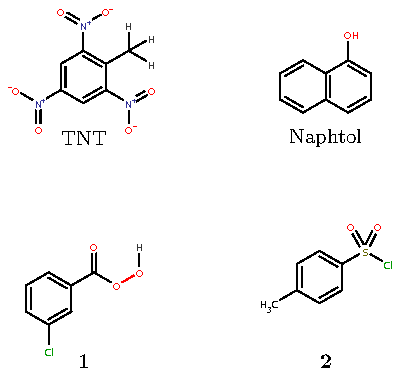
\includegraphics{fig3-2.pdf}
    \caption{Overlaying \LaTeX\ commands to get some nice things.}
    \label{fig:struct1}
\end{figure}

%
You can check out the code listing for creating the figure \ref{fig:struct1}
    bellow:
    \lstinputlisting{fig3-2.tex}

%
\begin{figure}[h]
    \centering
    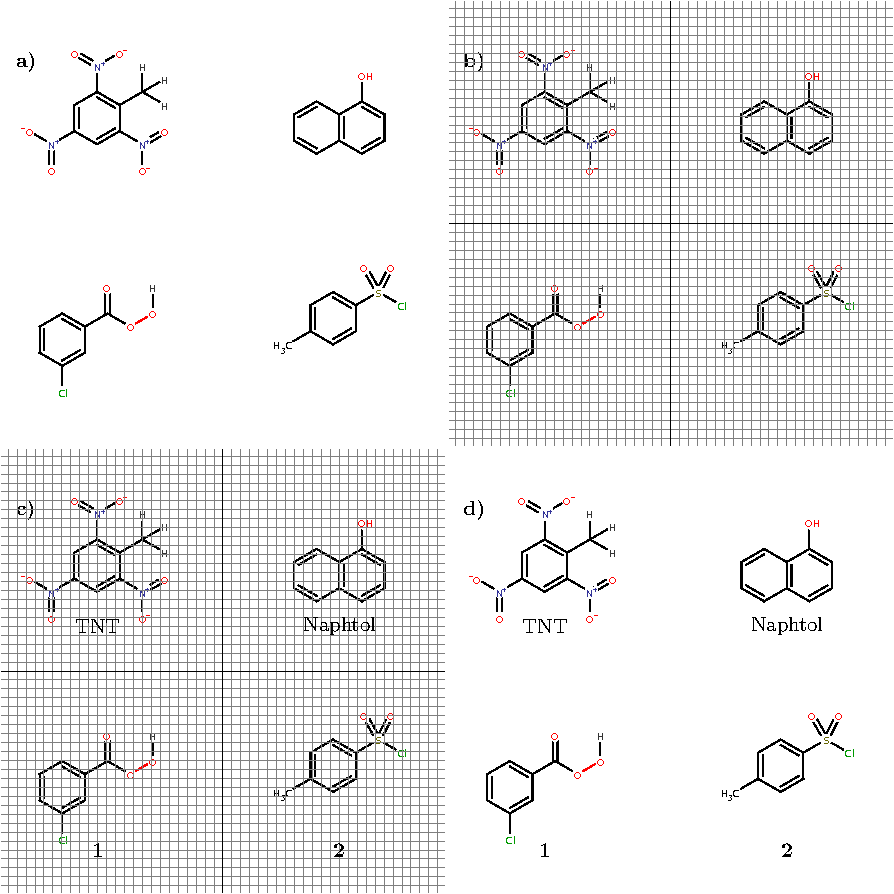
\includegraphics{fig3-1.pdf}
    \caption{
    The work-flow how figure annotation using \pkg{TikZ} is done.
    %
    Part \textbf{a)} shows just a plain figure before annotation, where the
        later steps (\textbf{b)} and \textbf{c)}) involve drawing a grid and the
        positioning the labels at the right positions.
    %
    And \textbf{d)} shows the image after the grid was removed.
    %
    NB this illustration was done also using the very same \pkg{TikZ} package.}
    \label{fig:struct1multi} 
\end{figure}
%
This way one can create good figures very easily.
%
What is more, if you have just simple structure images you do not have to worry
    about placing them correctly using your mouse or making sure that the font
    will be the same as in all the other text if you overlay everything using
    this \LaTeX{} package.

%
\clearpage
\subsubsection{Example 2: Composing a Scheme of Individual Structures}

%
In this example I have used a scheme by Eric Appel to extract the structures of
    the compounds and then I have put all the annotations using TikZ macros.
%
This way allows the user to use the same type of lines consistently throughout
    all figures and the most importantly it allows to ensure, that the figures
    remains scaled by the same factor.
%
You can see, that I have slightly scaled down the figures above the arrow and
    the scaling factor there is $4/5$, but most importantly, all the figures
    will be scaled the same way, because I have created a common style for them.

%
Another very good thing is that I have made this figure in a special
\env{standalone} environment and this lets me do two things:
\begin{enumerate}
    \item
        Compile only the figure, which lets me to preview it as a separate
            \ftype{pdf} file and since the compilation time is decreased, I can
            create it faster.
        %
    \item
        Include the whole \ftype{tex} file in the document via \cmd{input}
            command, so that I can get all cross-references right.
\end{enumerate}

%
\begin{figure}[h]
    \centering
    \textbf{Original:}\\
    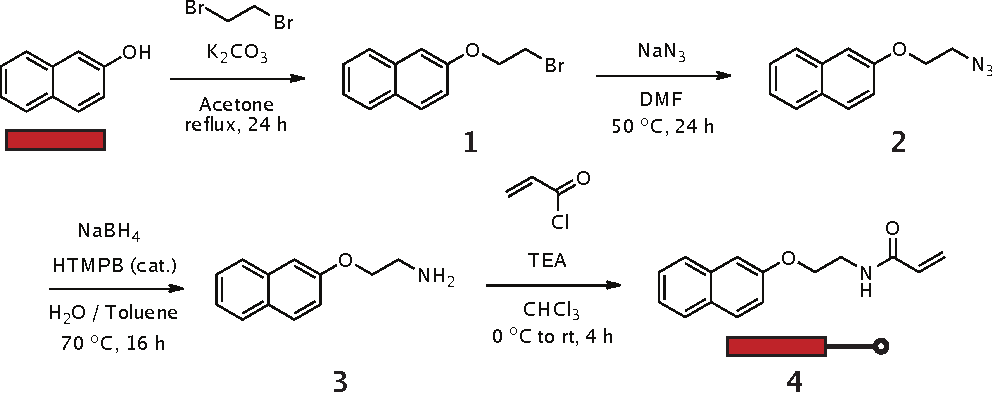
\includegraphics[scale=.9]{scheme-all.pdf}
    \vskip .5em\hrule\vskip 1em
    \textbf{Tikz:}\\
    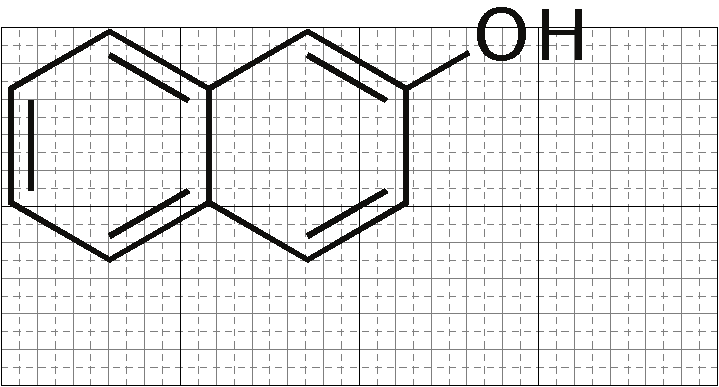
\includegraphics{fig4.pdf}
    \caption{Comparison of two figures, one created with ChemDraw and Adobe
        Illustrator by Eric Appel, whereas another, was created by me just using
        the chemical structures as images and putting them into right order.
        All the annotations where done in LaTeX and both figures are not
        scaled.}
    \label{fig:scheme}
\end{figure}
\todo{Try to make the scheme in fig \ref{fig:scheme} look nicer}

%
The code for the figure can be found in the \fname{fig4}{tex} in the same
    directory as the sources of this tutorial.
%
There are several differences in style of composing the figure while compared
    with the previous \pkg{TikZ} example.
%
To begin with, the previous example used absolute positions and it might have
    probably been better to use \pkg{overpic} package, if I needed just to
    overlay some text.
%
However, this example did not use absolute positions at all and everything is
    done via different nodes and relative positioning.
%
This concept might be slightly harder from the first look, but it is actually
    much easier to write, that \cmd{img1} will be to the left of \cmd{img2} and
    in between there will be an arrow.
%
The source code of the figure is documented with further comments, should you
    want any more explanation on the executed commands.

My drawn example is just a proof of concept and I think that with a bit of
    effort it can be made to look even better, but I just did not want to spend
    too much time on this.
%
However, one can note very easily, that the fonts in the structures are not the
    same as the surrounding annotations.
%
The solution to this is described in the next sub-sub-section.

%
\clearpage
\subsubsection{Example 3: Using \pkg{ChemFig} Package to Draw 2D Structures}

%
The third example shows third case scenario, where one might want to create
    entire structures using \LaTeX{} macros.
%
For this job I chose to use the \pkg{ChemFig} package, which is just a set of
    macros for the \pkg{TikZ} package, which ease the creation of 2D structures.
%
I have redraw the structures used earlier (fig. \ref{fig:struct1}), which for
    me did not look right, as the text was way too small and the alignment was
    not perfect.

%
This time, using \pkg{ChemFig} and \pkg{TikZ} I could create much nicer figures,
    and for those who are worrying about how much time it takes, I can answer,
    that it actually takes less time to get this perfectly looking figure, than
    trying to make your software use the same fonts you use in your document and
    then overlay the figure with text.
%
The results are shown in the figure \ref{fig:chemfig}.

\begin{figure}[htpb]
    \centering
    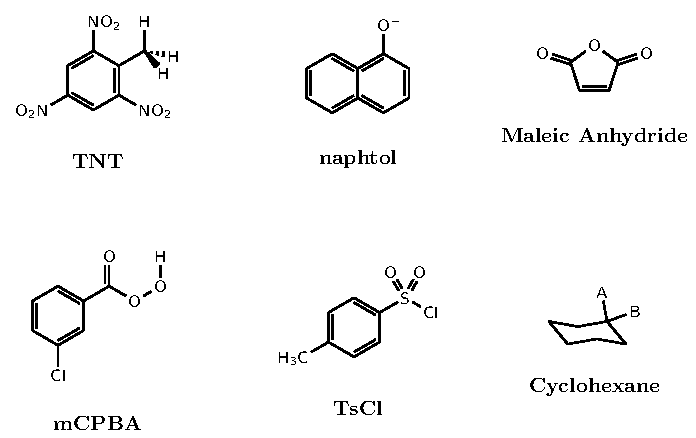
\includegraphics{fig5.pdf}
%    \documentclass{standalone}
\usepackage{tikz,amsmath,graphicx,calc,chemfig}
\usepackage[update,verbose=false]{epstopdf}
\usepackage[version=3]{mhchem}
\graphicspath{{./figs/}}
\usetikzlibrary{
    arrows,
    decorations.pathmorphing,
    backgrounds,
    positioning,
    fit,
    petri
}
\setatomsep{5mm}
\setbondoffset{.5mm}
\setcrambond{2.5pt}{1pt}{2pt}
\setbondstyle{thick}
\renewcommand*\printatom[1]{{\footnotesize\ensuremath{\mathsf{#1}}}}
\definesubmol{no2}{*6(-\chemabove{N}{+}(=O)-O\rlap{${}^{-}$})}


\begin{document}
\begin{tikzpicture}
    [scale=1,
     structure/.style={rectangle,draw=white,fill=white,
               outer xsep=.2cm,outer ysep=.2cm,minimum size=2mm,node distance=1.4cm},
     label/.style={rectangle,fill=white,font=\bfseries,
               outer ysep=.2cm,minimum size=4mm,},
     arrow/.style={->,>=stealth',semithick},
     reagent/.style={text width=2cm,font=\footnotesize,align=center,midway},
     designbox/.style={rectangle,draw=black,thick,fill=red,
               inner sep=0pt,minimum width=15mm, minimum height=2.5mm, node distance=0mm}]
    %
    \matrix[column sep=1.4cm,row sep=2cm]{
        \node[structure] (TNT)       {\chemfig{*6((-O_2N)=-(-NO_2)=(-(<[::-80]H)(<:[::-40]H)(-[::60]H))-(-NO_2)=-)}}; &
        \node[structure] (naphtol)   {\chemfig{*6(-=*6(=-=-(-O\rlap{${}^{-}$})=)-=-=)}}; &
        \node[structure] (MalAnh)    {\chemfig{[:18]*5(=-[::60](=O)-O-[::60](=O)-)}}; \\
        \node[structure] (mCPBA)     {\chemfig{*6(-(-Cl)=-*6(-*6(-O-O-H)=O)=-=)}}; &
        \node[structure] (TsCl)      {\chemfig{*6((-H_3C)-=-(-S([:120]=O)([:60]=O)-[:-30]Cl)=-=)}}; &
        \node[structure] (Hex-chair) {\chemfig{?-[:-50]-[:10]-[:-10]-[:130](-[:20]B)(-[:100]A)-[:190]?}}; \\
    };

    \draw (TNT.south)      node[label,yshift=-0.4cm]{TNT};
    \draw (naphtol.south)  node[label,yshift=-0.4cm]{naphtol};
    \draw (mCPBA.south)    node[label,yshift=-0.4cm]{mCPBA};
    \draw (TsCl.south)     node[label,yshift=-0.4cm]{TsCl};
    \draw (MalAnh.south)   node[label,yshift=-0.4cm]{Maleic Anhydride};
    \draw (Hex-chair.south)node[label,yshift=-0.4cm]{Cyclohexane};
\end{tikzpicture}
\end{document}

    \caption{
    \pkg{ChemFig} and \pkg{TikZ} usage to create very good-looking
        figures.
    %
    Note that the charge signs are different, and this is just to
        show different options, which are provided by this package.}
    \label{fig:chemfig}
\end{figure}

%
In my opinion this is the best way to produce good looking structures and in my
    experience it has only one glitch, where it has problems with positioning
    text containing superscripts and subscripts (as said in the documentation).
%
However, I do think, that it is not impossible to fix it and it should get
    improved soon.

% ----------------------------------------------------------------------
\clearpage
\section{Substituting Postscript Code with \LaTeX{} Macros}
% ----------------------------------------------------------------------

%
Another way to modify graphics is to use packages, which ease the replacement of
    the Postscript code into \LaTeX{} commands, which gives you a lot of control
    on the looks of your figures.
%
However, one must need to use a standard \verb|latex| compiler to leverage this
    functionality, because otherwise, the \ftype{eps} figures will not be
    post-processed by \TeX{}.
%
On the other hand, that was true only until recently when some people thought of
    packages, which go around these limitations and psfrag-like substitution
    becomes available using all compilers.

\comment{
%
This approach gives you those nice fonts, which \LaTeX{} uses and one can
    achieve very consistent looks over the entire document.
%
What is more, you can replace the Poscript code with your own created macros,
    which might be very useful if you want to cross-reference some objects
    inside the figures.
    }

%
\subsection{The \pkg{psfrag} package}

%
The mechanism of how this package works is very simple.
%
You create markers inside a \ftype{eps} figure (e.g. TMP1, or TMP2) and then
    replace them with \LaTeX{} macros by issuing the following command inside
    the figure environment, but before \verb|includegraphics| command:
%
\begin{lstlisting}
\psfrag{tag}[position][psposition][scale][rotation]{LaTeX construction}
\end{lstlisting}

%
You can deduce, that with this approach one can get the same font-faces, which
    are being used by \LaTeX{} and, what is more, the font sizes are retained
    the same as in the .eps figure, so you are not tied to the \cmd{normalsize}
    or \cmd{footnotesize} font sizes.
%
Although this might come handy at times, my personal opinion is that with more
    flexibility one can introduce more inconsistencies.
%
Hence, one should avoid fiddling with the font-sizes a lot unless it is
    necessary and everything should be defined via macros such as
    \cmd{normalsize}, \cmd{tiny}, \cmd{footnotesize} and similar.

%
\subsection{The \pkg{pstool} package}

%
This is one of the packages, which let you use \pkg{psfrag} type functionality
    without sacrificing the advantages of \pkg{pdflatex} compiler.
%
It basically processes the figures separately before including the as already
    processed \ftype{pdf} files and one can get most of the psfrag functionality
    this way.

%
Another advantage of this approach is that the figures are processes only when
    needed and the compilation times decrease.

%
\subsection{The \pkg{pst-pdf} package}

%
This package does similar thing as \pkg{pstool}, but where the first is striving
    to provide functionality of the \pkg{psfrag} package, the \pkg{pst-pdf}
    package is for dealing with \pkg{pstricks} routines.
%
The mechanism of how it is done, is basically very similar to the approach
    described above.
    \todo{Links to the documentation}


% ----------------------------------------------------------------------
\end{document}
% ----------------------------------------------------------------------

% Editor configuration:
% vim: tw=80:spell:spelllang=en_gb
